% Exercise Template
% A LaTeX template for typesetting exercise in Persian (with cover page).
% By: Reza Adinepour
% Github: github.com/rezaAdinepour

\documentclass[12pt]{exam}

\usepackage{setspace}
\usepackage{listings}
\usepackage{graphicx,wrapfig}
\usepackage{caption}
\usepackage{subcaption}
\usepackage{multirow}
\usepackage{matlab-prettifier}
\usepackage{amsmath}
\usepackage{multicol}
\usepackage[hidelinks]{hyperref}



\usepackage[utf8]{inputenc}
\usepackage{fourier} 
\usepackage{array}
\usepackage{makecell}

\renewcommand\theadalign{bc}
\renewcommand\theadfont{\normalsize}
\renewcommand\theadgape{\Gape[4pt]}
\renewcommand\cellgape{\Gape[4pt]}


\usepackage[margin=25mm]{geometry}
\usepackage{xepersian}
\settextfont{XB Niloofar}

\newcommand{\class}{\ThesisClass}

\singlespacing
\parindent 0ex

\begin{document}


% -------------------------------------------------------
%  Thesis Information
% -------------------------------------------------------

\newcommand{\ThesisType}
{سمینار}  % پایان‌نامه / رساله
\newcommand{\ThesisDegree}
{کارشناسی ارشد گرایش معماری کامپیوتر}  % کارشناسی / کارشناسی ارشد / دکتری
\newcommand{\ThesisMajor}
{مهندسی کامپیوتر}  % مهندسی کامپیوتر
\newcommand{\ThesisTitle}
{تمرین شبیه‌سازی سری ۳}
\newcommand{\ThesisAuthor}
{\href{https://github.com/rezaAdinepour/M.Sc-AUT/tree/main/Advanced Computer Architecture}{\textcolor{black}{رضا آدینه پور}} - ۴۰۲۱۳۱۰۵۵}
\newcommand{\ThesisSupervisor}
{جناب آقای دکتر فربه}
\newcommand{\ThesisDate}
{۲۳ آذر ۱۴۰۲}
\newcommand{\ThesisDepartment}
{دانشکده مهندسی کامپیوتر}
%\newcommand{\ThesisUniversity}
%{دانشگاه صنعتی امیرکبیر}

% -------------------------------------------------------
%  English Information
% -------------------------------------------------------

%\newcommand{\EnglishThesisTitle}{A Standard Template for Course Exercise}


\pagestyle{empty}

\begin{center}


\includegraphics[scale=0.15]{images/aut-fa.png}

%\vspace{0.5cm}
%\ThesisUniversity \\[-0.3em]
%\vspace{0.5cm}
\large\ThesisDepartment

\begin{large}
\vspace{0.5cm}


%\ThesisMajor

\end{large}

\vspace{1.5cm}

{عنوان:}\\[1.2em]
{\LARGE\textbf{\ThesisTitle}}\\ 
\vspace{1cm}
% \begin{latin}
% {\Large\textbf\EnglishThesisTitle}
% \end{latin}

\vspace{2cm}

{نگارش}\\[.5em]
{\large\textbf{\ThesisAuthor}}

\vspace{1.5cm}

{استاد مربوطه}\\[.5em]
{\large\textbf{\ThesisSupervisor}}

\vspace{1cm}



\vspace{2cm}

\ThesisDate

\end{center}

\newpage


% These commands set up the running header on the top of the exam pages
\pagestyle{head}
\firstpageheader{}{}{}
\runningheader{صفحه \thepage\ از \numpages}{}{\class}
\runningheadrule

\vspace{0pt}


\begin{questions}
	\pointpoints{نمره}{نمره}
	
	
	\question
	\textbf{فرض کنید یک شرکت صنعتی می خواهد برای یک کاربرد پردازش تصویر، یک شتاب دهنده سخت افزاری که بیس آن شبکه CNN است طراحی کنید. مزایا و معایب استفاده از DRAM یا SRAM را به عنوان حافظه جانبی این شتاب‌دهنده بررسی کنید و درمورد آن بحث کنید.}
	
	
	
	انتخاب میان DRAM و SRAM به پارامتر‌های بسیار زیادی بستگی دارد که در ادامه چند مورد از آنها را بررسی و باهم مقایسه می‌کنیم.
	
	برای مثال زمان خواندن و نوشتن از حافظه برای ما مهم است. در این اپلیکیشن که نیاز است داده ها به صورت RealTime نوشته و از حافظه خوانده شود این قضیه بسیار مهم است و نیازمند حافظه ای هستیم که کمترین تاخیر در خواندن و نوشتن را داشته باشد. از میان SRAM و DRAM ،‌ حافظه SRAM زمان دسترسی کمتری را بریا ما فراهم می‌کند. بنابر این با درنظر گرفتن زمان دسترسی،‌ انتخاب پیشنهادی بنده به این شرکت،‌ حافظه های مبتنی بر SRAM است.
	
	
	توان مصرفی حافظه نیز یکی از پارامتر های مهم در انتخاب حافظه است. به طور کلی حافظه های مبتنی بر DRAM مصرف توان کمتری نسبت به SRAM ها دارند. چرا که فقط در زمان خواندن و نوشتن نیاز به تغذیه دارند اما SRAM ها برای نگه داشتن دیتا همواره نیاز به وصل بودن تغذیه دارند. بنابر این  اگر محصول این شرکت به گونه ای باشد که می‌بایست با باتری کوچکی برای مدتی طولانی کار کند، نیاز مند آن است که از DRAM استفاده کنند.
	
	حافظه های مبتنی بر SRAM چگالی بیشتری نسبت به DRAM ها دارند. چگالی بدین معنا که در مساحت یکسان، تعداد سلول های SRAM بیشتری را می‌توان در کنار هم قرار داد و در نتیجه مقدار حافظه بزرگتری به ازای مساحت یکسانی داریم. density کمتر DRAM ها عمدتا به دلیل خازن های نگه دارنده بیت هاست چرا که اندازه ان را نمی‌توان از یک مقدار کمتر کنیم. بنابر این در این کاربرد با توجه به مساحت در دسترس تراشه و مقدار حافظه مورد نیاز که بر اساس تعداد لایه های شبکه CNN و بار محاسبات انجامی تعیین می‌شود می‌توان نوع حافظه مورد نیاز را تعیین کرد.
	

دیدگاه بعدی ای که می‌توان به این مسئله نگاه کرد بدین صورت است که آیا شبکه قرار است همواره Train شود یا خیر. اگر قرار باشد شبکه به صورت بلادرنگ Train شود، شاید بهتر باشد که از DRAM استفاده کرد چرا که DRAM برای نگه داشتن مقادیر خود نیاز به Refresh شدن دارد بنابر این می‌توان با تغییر وزن ها و آپدیت شدن آنها با آموزش جدید، Refresh شوند. البته این نکته را باید ذکر کرد که در این شرایط توان مصرفی شبکه وحشتناک زیاد می‌شود و دیگر نمی‌توان آن را با باتری کوچکی راه اندازی کردو چرا که شبکه مدام Train می‌شود و وزن های خودش را بر اساس شرایط و مسئله ای که با آن مواجه است آپدیت می‌کند و این امر نیازمند انرژی زیادی است.


بنا بر این با توجه به نکات گفته شده، می‌توان بر اساس جزئیات دقیق مسئله که ما اطلاعی از آن نداریم، یکی از حافظه‌های SRAM یا DRAM را انتخاب کنیم.
	
	
	\question
	\begin{enumerate}
		\item \textbf{بانک مموری ۳×۳ با استفاده از سلول SRAM ۶ ترانزیستوری همراه با SenseAmplifier طراحی کنید.}
		
		
		
		برای طراحی بانک مموری، ابتدا یک سلول SRAM ۶ ترانزیستوری را طراحی می‌کنیم.
		
		شماتیک مدار طراحی شده به صورت زیر است:
		
		\begin{figure}[h]
			\centering
			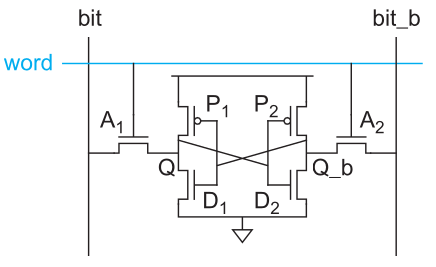
\includegraphics[width=0.6\textwidth]{images/img1}
			\caption{سلول ۶ ترانزیستوری SRAM}
			\label{سلول ۶ ترانزیستوری SRAM}
		\end{figure}
		
		
		
\begin{latin}
	\texttt{.include '../Library/cmos45.lib'}\\\\
	\texttt{*************** circuits ***************}\\
	\texttt{.SUBCKT SRAM\_cell WL BL BLB Q QB}\\
	\texttt{* D G S}\\\\
	\texttt{M1 QB Q gnd gnd nmos L= '2*lambda' W= '8*lambda'}\\
	\texttt{M2 QB Q Vdd Vdd pmos L='2*lambda' W='10*lambda'}\\
	\texttt{M3 Q QB gnd gnd nmos L= '2*lambda' W= '8*lambda'}\\
	\texttt{M4 Q QB Vdd Vdd pmos L='2*lambda' W='10*lambda'}\\
	\texttt{M5 QB WL BLB gnd nmos L= '2*lambda' W= '4*lambda'}\\
	\texttt{M6 BL WL Q gnd nmos L= '2*lambda' W= '4*lambda'}\\\\
	\texttt{.ends}\\
\end{latin}


در این طراحی از از کتابخانه \texttt{cmos45.lib} استفاده شده است. و نسبت $\frac{W}{L}$ ترانزیستور ها با سعی و خطا بدست آورده شده است.

کد نوشته شده برای تک سلول SRAM درون فایل \texttt{tb\_cell.sp} تست شده است. که به دلیل طولانی بودن کد آن را در گزارش نیاورده اینم.

برای طراحی مدار کنترلی و جانبی این طراحی، یک دیکدر ۲ به ۴ استفاده شده است که یکی از خروجی های آن بلا استفاده است.

کد نوشته شده برای مدار دیکدر به صورت زیر است:
\begin{latin}
	 \texttt{*************** circuits ***************}\\
	 
	 \texttt{.subckt DECODER in1 in2 in1! in2! out1 out2 out3 out4}\\
	 
	 \texttt{*** line 1 ***}\\
	 \texttt{MN11 out1 in1 0   0   NMOS  L='2*lambda' W='4*lambda'}\\
	 \texttt{MN12 out1 in2 0   0   NMOS  L='2*lambda' W='4*lambda'}\\
	 \texttt{MP1  out1 0   vdd vdd PMOS  L='2*lambda' W='10*lambda'}\\
	 
	 \texttt{*** line 2 ***}\\
	 \texttt{MN21 out2 in1! gnd gnd NMOS  L='2*lambda' W='4*lambda'}\\
	 \texttt{MN22 out2 in2  gnd gnd NMOS  L='2*lambda' W='4*lambda'}\\
	 \texttt{MP2  out2 gnd  vdd vdd PMOS  L='2*lambda' W='10*lambda'}\\
	 
	 \texttt{*** line 3 ***}\\
	 \texttt{MN31  out3 in1  gnd gnd NMOS  L='2*lambda' W='4*lambda'}\\
	 \texttt{MN32  out3 in2! gnd gnd NMOS  L='2*lambda' W='4*lambda'}\\
	 \texttt{MP3   out3 gnd  vdd vdd PMOS  L='2*lambda' W='10*lambda'}\\
	 
	 \texttt{*** line 4 ***}\\
	 \texttt{MN41  out4 in1! gnd gnd NMOS  L='2*lambda' W='4*lambda'}\\
	 \texttt{MN42  out4 in2! gnd gnd NMOS  L='2*lambda' W='4*lambda'}\\
	 \texttt{MP4   out4 gnd  vdd vdd PMOS  L='2*lambda' W='10*lambda'}\\
	 
	 \texttt{.ends}
\end{latin}

تست بنچ این مدار نیز در فایل \texttt{tb\_decoder.sp} موجود است.

در نهایت همه کد های نوشته شده را در فایل \texttt{main.sp} اضافه می‌کنیم و بانک حافظه ۳×۳ را شبیه‌سازی می‌کنیم.

خروجی شبیه سازی برای یک سیکل نوشتن و خواندن به صورت «شکل \textcolor{blue}{\ref*{خروجی شبیه‌سازی بانک مموری SRAM}}» است.

\begin{figure}[h]
	\centering
	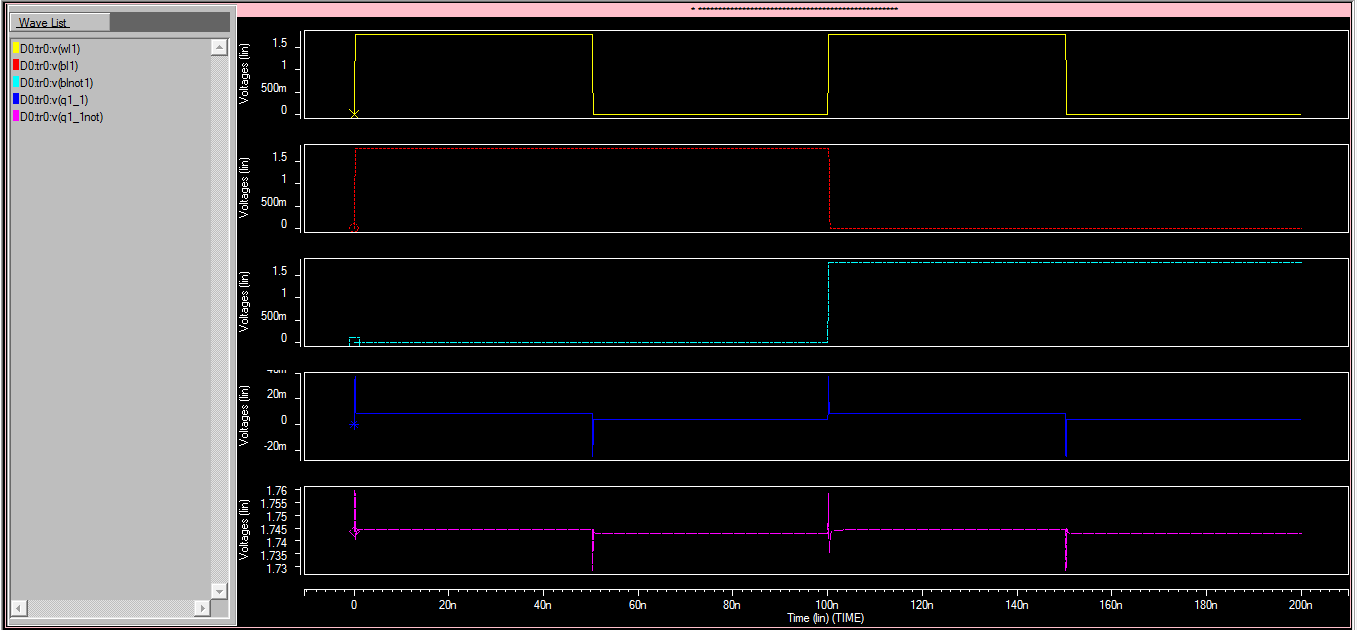
\includegraphics[width=1\textwidth]{images/img2}
	\caption{خروجی شبیه‌سازی بانک مموری SRAM}
	\label{خروجی شبیه‌سازی بانک مموری SRAM}
\end{figure}




		
		
		
		
		
		
		
		
		
		
		
		
		
		
		
		
		\item \textbf{بانک مموری ۳×۳ با استفاده از سلول DRAM ۶ ترانزیستوری همراه با SenseAmplifier طراحی کنید.}
	\end{enumerate}
	
	
	سلول DRAM طراحی شده به صورت «شکل \textcolor{blue}{\ref*{سلول DRAM}}» است.
	
	\begin{figure}[h]
		\centering
		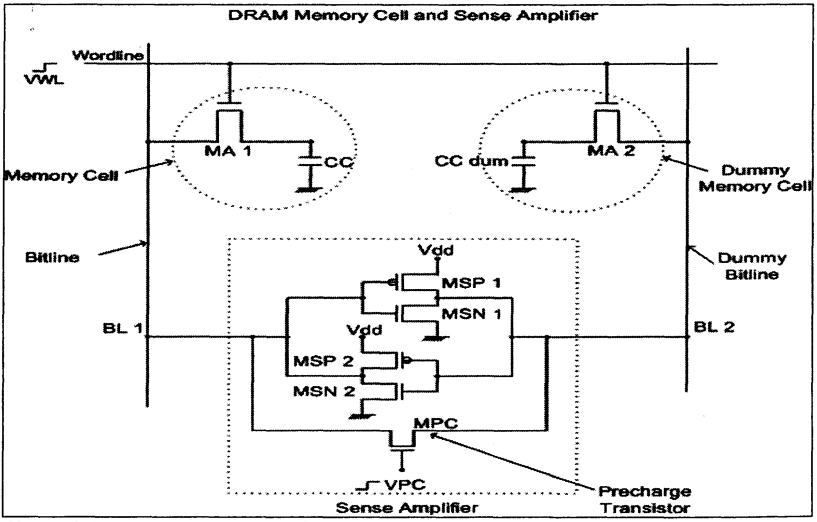
\includegraphics[width=0.7\textwidth]{images/img3}
		\caption{سلول DRAM}
		\label{سلول DRAM}
	\end{figure}
	
	
	کد نوشته شده برای سلول DRAM به صورت زیر است:
	
	
	\begin{latin}
		\texttt{********** circuit **********}
		
		\texttt{.SUBCKT DRAM\_cell WL BL BLB VPS}\\
		\texttt{VDD 3 0 DC 3}\\
		\texttt{CBL1 BL 0 100fF}\\
		\texttt{CBL2 BLB 0 100fF}\\\\
		\texttt{* cell}\\
		\texttt{MA1 BL WL 1 0 nmos W=0.3u L=0.2u}\\
		\texttt{CC 1 0 50FF}\\
		\texttt{MA2 BLB WL 7 0 nmos W=0.3u L=0.2u}\\
		\texttt{CCdum 7 0 50fF}\\
		
		\texttt{*sense amplifier}\\
		\texttt{MSN1 BLB BL 0 0 nmos W=0.952u L=0.18u}\\
		\texttt{MSP1 BLB BL 3 3 pmos W=2u L=0.18u}\\
		\texttt{MSN2 BL BLB 0 0 nmos W=0.952u L=0.18u}\\
		\texttt{MSP2 BL BLB 3 3 pmos W=2u L=0.18u}\\
		\texttt{MPC BL VPS BLB 0 nmos W=1.62u L=0.18u}\\
		
		\texttt{.ends}\\
	\end{latin}
	
	 در این کد نیز از کتابخانه \texttt{cmos45.lib} استفاده شده است. و همچنین تست‌بنچ این طراحی نیز در فایل \texttt{tb\_Cell} نوشته شده است.
	 
	 مدار جانبی و کنترلی این طراحی نیز، همان دیکدر قسمت قبل است. بنابر این از آوردن مجدد کد خودداری می‌کنیم.
	 
	 بانک مموری DRAM در فایل \texttt{main.sp} نوشته شده است.
	 
	 خروجی این شبیه سازی به صورت «شکل \textcolor{blue}{\ref{خروجی شبیه‌سازی بانک مموری DRAM}}» است.
	 
	 \begin{figure}[h]
	 	\centering
	 	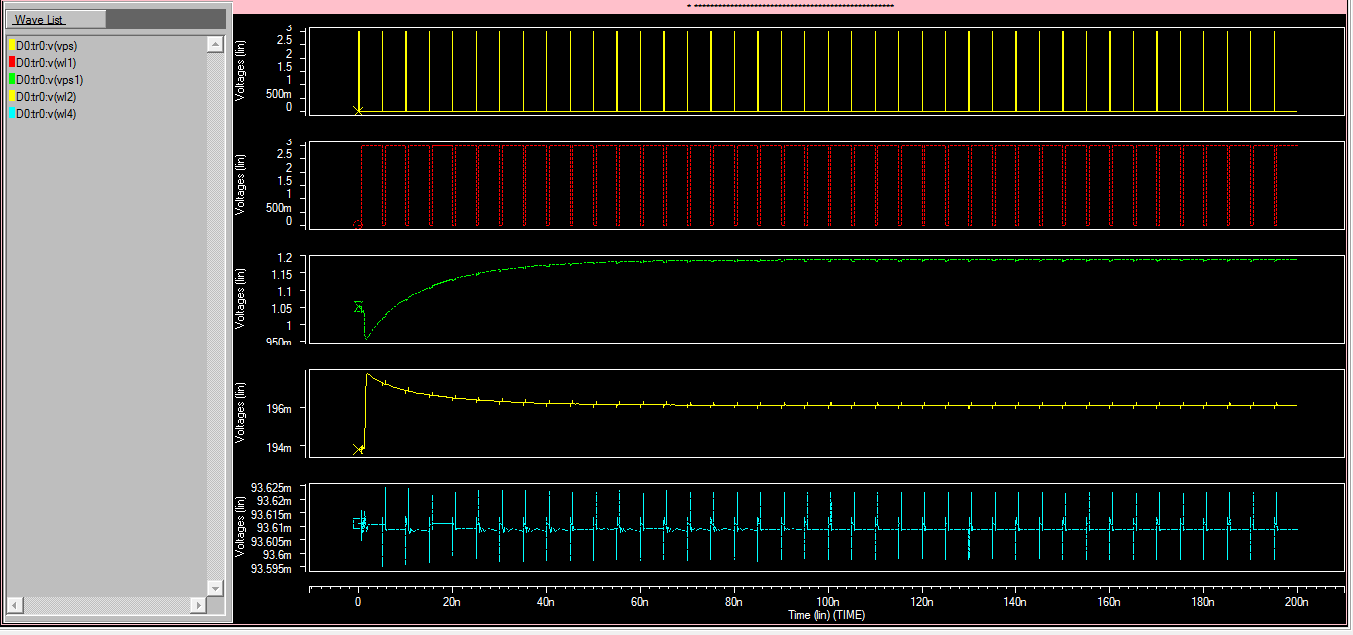
\includegraphics[width=1\textwidth]{images/img4}
	 	\caption{خروجی شبیه‌سازی بانک مموری DRAM}
	 	\label{خروجی شبیه‌سازی بانک مموری DRAM}
	 \end{figure}
	 
	 
	 بر اساس خروجی‌های شبیه سازی که در فایلی با پسوند \texttt{.lis} ذخیره می‌شوند. می‌توان جدول زیر را تکمیل کرد.
	 
	 بر اساس خروجی های بدست آمده می‌توان مشاهده کرد که عملکرد SRAM نسبت به DRAM از نظر توان مصرفی و زمان نوشتن بهتر است. این انتظار را داشتیم. چرا که در سلول DRAM نیاز به Refresh داریم و این کار باعث عبود جریان بیشتری از مدار (در زمان یکسان) می‌شود. بنابراین انتظار می‌رود توان مصرفی آن نیز بیشتر باشد. که خروجی شبیه‌سازی نیز این را اثبات می‌کند.
	 
	 
	 
	 \begin{latin}
	 	 \begin{center}
	 	 	\begin{tabular}{||c c c||} 
	 	 		\hline
	 	 		& SRAM & DRAM  \\[0.5ex]
	 	 		\hline\hline
	 	 		Read time & 0.08s & 0.08s \\
	 	 		\hline
	 	 		Write time & 0.43s & 33.90s \\
	 	 		\hline
	 	 		Total power & 2.0593 mW & 20.0425mW \\ [0.5ex] 
	 	 		\hline
	 	 	\end{tabular}
	 	 \end{center}
	 \end{latin}
	 
	
 
 \end{questions}

\end{document}